\section{Resultados}

\subsection{Comparación en el periodo de desarrollo (2015--2018)}

La tabla \ref{tab:global} compara los procedimientos con el NMAE macro en las ventanas W1--W3 (validaciones de 2016, 2017 y 2018). Estas cifras corresponden al \textbf{periodo de desarrollo (2015--2018)}; la reserva de 2019 se presenta por separado en la sección \ref{sec:final}. La última fila es el Random Forest con calendario cíclico (M3$^\ast$), definido en la sección \ref{sec:sens}.

\begin{table}[!htbp]
    \centering
        \caption{NMAE macro por ventana de validación (adimensional), promedio y desviación estándar entre ventanas (descriptiva: las ventanas comparten datos de entrenamiento), y cambio relativo del promedio frente a la referencia estacional semanal.}
        \label{tab:global}
        \footnotesize
        \begin{tabular}{lrrrrrr}
\toprule
Procedimiento & W1 & W2 & W3 & Media & Desv. est. entre ventanas & Cambio vs. estacional \\
\midrule
Persistencia & 0{,}0677 & 0{,}0678 & 0{,}0683 & 0{,}0679 & 0{,}0003 & +26{,}4\% \\
Estacional semanal & 0{,}0501 & 0{,}0542 & 0{,}0569 & 0{,}0537 & 0{,}0034 & -- \\
\midrule
M1: Ridge & 0{,}0417 & 0{,}0428 & 0{,}0440 & 0{,}0428 & 0{,}0012 & -20{,}3\% \\
M2: Árbol podado & 0{,}0372 & 0{,}0363 & 0{,}0347 & 0{,}0361 & 0{,}0012 & -32{,}9\% \\
M3: Random Forest (dummies) & 0{,}0288 & 0{,}0286 & 0{,}0272 & 0{,}0282 & 0{,}0009 & -47{,}5\% \\
\textbf{M3$^\ast$: Random Forest (cíclico)} & 0{,}0276 & 0{,}0275 & 0{,}0262 & 0{,}0271 & 0{,}0007 & -49{,}6\% \\
\bottomrule
\end{tabular}
\end{table}

Entre los procedimientos originales, el Random Forest con indicadores (M3) es el mejor en las tres ventanas (0,0282) y reduce el error 47,5\,\% frente a la referencia semanal, 34,1\,\% frente a Ridge y 21,8\,\% frente al árbol podado. Su ventaja crece de W1 a W3 porque la referencia empeora (0,0501 a 0,0569). M3 es el mejor también en cada país (anexo, tabla \ref{tab:detalle}); Francia es el más difícil y su referencia semanal rinde peor que la persistencia. No se investigó la causa; una hipótesis, no evaluada, es su estacionalidad más marcada (anexo, figura \ref{img:descriptiva}) y una mayor dependencia de la temperatura, que el modelo no observa.

\textbf{Complejidad, costo e interpretabilidad.} Ridge es el más simple e interpretable y el menos preciso; el árbol podado final tiene 4\,261 hojas y el Random Forest cíclico 200 árboles y 11,4 millones de nodos, con ajuste final de 8,5 s (142 s con indicadores y 70 s el árbol; anexo, tablas \ref{tab:complejidad} y \ref{tab:tiempos}). En el bosque, \texttt{lag\_168h} (64,7\,\%), \texttt{demand\_mw} (24,7\,\%) y \texttt{lag\_48h} (5,0\,\%) concentran la importancia por impureza, que se interpreta con cautela por la correlación entre predictores.

\subsection{Análisis de sensibilidad} \label{sec:sens}

Ambos análisis se definen y evalúan solo en el periodo de desarrollo (2015--2018), con las mismas ventanas y métrica, y con los hiperparámetros de M1 y M3 fijos (tabla \ref{tab:busqueda}); se evalúa el efecto de la decisión, no de una nueva búsqueda (tabla \ref{tab:sens}).

\begin{table}[!htbp]
    \centering
        \caption{NMAE macro por ventana en los análisis de sensibilidad (Ridge y Random Forest) y cambio relativo del promedio frente al escenario base.\label{tab:sens}}
        \small
        \begin{tabular}{llrrrrr}
\toprule
Análisis & Escenario & W1 & W2 & W3 & Promedio & Cambio vs. base \\
\midrule
S1: calendario & Random Forest, dummies (base) & 0{,}0288 & 0{,}0286 & 0{,}0272 & 0{,}0282 & -- \\
 & Random Forest, cíclico & 0{,}0276 & 0{,}0275 & 0{,}0262 & 0{,}0271 & -3{,}9\% \\
S1: calendario & Ridge, dummies (base) & 0{,}0417 & 0{,}0428 & 0{,}0440 & 0{,}0428 & -- \\
 & Ridge, cíclico & 0{,}0467 & 0{,}0472 & 0{,}0487 & 0{,}0475 & +11{,}0\% \\
\midrule
S2: historia$^\dagger$ & Random Forest, ventana creciente (base) & 0{,}0288 & 0{,}0286 & 0{,}0272 & 0{,}0279 & -- \\
 & Random Forest, último año & 0{,}0288 & 0{,}0309 & 0{,}0296 & 0{,}0302 & +8{,}3\% \\
S2: historia$^\dagger$ & Ridge, ventana creciente (base) & 0{,}0417 & 0{,}0428 & 0{,}0440 & 0{,}0434 & -- \\
 & Ridge, último año & 0{,}0417 & 0{,}0427 & 0{,}0442 & 0{,}0435 & +0{,}2\% \\
\bottomrule
\end{tabular}
    \\ $^\dagger$ En W1 ambos esquemas de historia coinciden (solo existe 2015), por lo que el promedio y el cambio de S2 usan W2 y W3.
\end{table}

\textbf{S1: representación del calendario.} Se reemplazan los indicadores de hora, día y mes por pares seno--coseno con periodos 24, 7 y 12 (determinista, sin fuga). En el Random Forest el NMAE baja de 0,0282 a 0,0271 (3,9\,\%) y mejora en las tres ventanas; en Ridge sube de 0,0428 a 0,0475 (11,0\,\%), plausiblemente porque un solo seno y coseno por variable es demasiado rígido para un modelo lineal. \textbf{Decisión:} se adopta el Random Forest cíclico (M3$^\ast$) como versión final, elegido con S1 en el periodo de desarrollo (2015--2018) y antes de examinar 2019; Ridge y el árbol conservan indicadores (el árbol no se probó con esta representación). El ordenamiento de los procedimientos no cambia.

\textbf{S2: historia de entrenamiento.} Se reemplaza la ventana creciente por una que usa solo el año anterior a cada validación. El Random Forest empeora de 0,0279 a 0,0302 (8,3\,\%) en W2 y W3 y Ridge no cambia (0,0434 frente a 0,0435), plausiblemente porque el bosque necesita más historia para aprender interacciones; conviene reajustar con toda la historia disponible.

\subsection{Evaluación final en la reserva 2019} \label{sec:final}

Se reajustó cada procedimiento con los 103\,680 casos completos de 2015--2018 y se evaluó una vez en 2019, con 26\,031 casos (8\,736 en DE, 8\,736 en ES y 8\,559 en FR). La tabla \ref{tab:test} compara los seis procedimientos y la tabla \ref{tab:test_rf} da MAE, RMSE y NMAE por país del Random Forest cíclico y la referencia; el detalle está en el anexo (tabla \ref{tab:test_detalle}).

\begin{table}[!htbp]
    \centering
        \caption{NMAE por país y macro en la reserva 2019 (adimensional) y NMAE macro del periodo de desarrollo (2015--2018; M3$^\ast$: promedio de W1--W3 de S1). Las cifras de 2019 no se usaron para elegir nada.\label{tab:test}}
        \footnotesize
        \resizebox{\textwidth}{!}{\begin{tabular}{lrrrrrr}
\toprule
Procedimiento & NMAE DE & NMAE ES & NMAE FR & NMAE macro 2019 & NMAE macro del periodo de desarrollo (2015--2018) & Cambio vs. estacional (2019) \\
\midrule
Persistencia & 0{,}0817 & 0{,}0619 & 0{,}0574 & 0{,}0670 & 0{,}0679 & +32{,}8\% \\
Estacional semanal & 0{,}0458 & 0{,}0437 & 0{,}0618 & 0{,}0505 & 0{,}0537 & -- \\
\midrule
M1: Ridge & 0{,}0418 & 0{,}0425 & 0{,}0386 & 0{,}0410 & 0{,}0428 & -18{,}8\% \\
M2: Árbol podado & 0{,}0319 & 0{,}0273 & 0{,}0406 & 0{,}0333 & 0{,}0361 & -34{,}1\% \\
M3: Random Forest (dummies) & 0{,}0257 & 0{,}0213 & 0{,}0314 & 0{,}0262 & 0{,}0282 & -48{,}2\% \\
\textbf{M3$^\ast$: Random Forest (cíclico)} & 0{,}0243 & 0{,}0203 & 0{,}0301 & \textbf{0{,}0249} & 0{,}0271 & -50{,}7\% \\
\bottomrule
\end{tabular}}
\end{table}

\begin{table}[!htbp]
    \centering
        \caption{Random Forest cíclico frente a la referencia estacional semanal en la reserva 2019: MAE y RMSE en MW, NMAE y denominadores ($n$).\label{tab:test_rf}}
        \small
        \begin{tabular}{lrrrrrrrr}
\toprule
 & & \multicolumn{2}{c}{MAE (MW)} & \multicolumn{2}{c}{RMSE (MW)} & \multicolumn{2}{c}{NMAE} & \\
\cmidrule(lr){3-4}\cmidrule(lr){5-6}\cmidrule(lr){7-8}
País & $n$ & Estac. & RF & Estac. & RF & Estac. & RF & Cambio \\
\midrule
DE & 8\,736 & 2\,559 & 1\,355 & 4\,469 & 2\,227 & 0{,}0458 & 0{,}0243 & $-$47{,}0\% \\
ES & 8\,736 & 1\,255 & 583 & 2\,002 & 1\,015 & 0{,}0437 & 0{,}0203 & $-$53{,}6\% \\
FR & 8\,559 & 3\,337 & 1\,626 & 4\,635 & 2\,403 & 0{,}0618 & 0{,}0301 & $-$51{,}3\% \\
\midrule
Macro & 26\,031 & -- & -- & -- & -- & 0{,}0505 & 0{,}0249 & $-$50{,}7\% \\
\bottomrule
\end{tabular}
    \\ ``Estac.'': referencia estacional semanal; ``RF'': Random Forest cíclico; cambio sobre el NMAE.
\end{table}

El Random Forest cíclico obtiene un NMAE macro de 0,0249 frente a 0,0505 de la referencia: 50,7\,\% menos, similar al 49,6\,\% del periodo de desarrollo (2015--2018). Es el mejor en los tres países (reducciones de 47,0\,\% en DE, 53,6\,\% en ES y 51,3\,\% en FR; MAE de 1\,355, 583 y 1\,626 MW), y el ordenamiento de los procedimientos es el del periodo de desarrollo (2015--2018). El error de 2019 es igual o menor que el del periodo de desarrollo (2015--2018) en todos (sin señales de sobreajuste a la validación), aunque 2019 puede ser un año algo más fácil (la referencia baja de 0,0537 a 0,0505); por eso conviene comparar la mejora relativa, que se mantiene.

\subsection{Incertidumbre de la diferencia con la referencia} \label{sec:boot}

Se usa un \textit{bootstrap por bloques} (Künsch, 1989): la unidad es la semana de 7 días (52 bloques en 2019) con los tres países juntos, lo que conserva la dependencia temporal y la coincidencia de fechas entre países. En cada una de 2\,000 réplicas (semilla 42) se toman 52 bloques con reemplazo y se recalcula la diferencia de NMAE macro. Las predicciones son fijas (no se reajusta), de modo que el intervalo es condicional al ajuste y no incluye la incertidumbre de selección ni de entrenamiento (tabla \ref{tab:boot}).

\begin{table}[!htbp]
    \centering
        \caption{Diferencia de NMAE entre el Random Forest cíclico (M3$^\ast$) y cada comparador en la reserva 2019, con intervalos de bootstrap por bloques semanales.\label{tab:boot}}
        \footnotesize
        \resizebox{\textwidth}{!}{\begin{tabular}{lrcrrc}
\toprule
Comparación (M3$^\ast$ menos el comparador) & $\Delta$ NMAE & IC 95\,\% de $\Delta$ & $P(\Delta\geq 0)$ & Mejora relativa & IC 95\,\% de la mejora \\
\midrule
Macro vs. estacional semanal & $-$0{,}0256 & [$-$0{,}0319; $-$0{,}0202] & $<0{,}001$ & 50{,}7\% & [45{,}4\%; 54{,}9\%] \\
\hspace{1em}DE & $-$0{,}0216 & [$-$0{,}0298; $-$0{,}0148] & $<0{,}001$ & 47{,}0\% & [38{,}4\%; 54{,}4\%] \\
\hspace{1em}ES & $-$0{,}0234 & [$-$0{,}0299; $-$0{,}0175] & $<0{,}001$ & 53{,}6\% & [46{,}5\%; 59{,}2\%] \\
\hspace{1em}FR & $-$0{,}0317 & [$-$0{,}0399; $-$0{,}0237] & $<0{,}001$ & 51{,}3\% & [44{,}6\%; 56{,}6\%] \\
\midrule
Macro vs. M1: Ridge & $-$0{,}0161 & [$-$0{,}0174; $-$0{,}0149] & $<0{,}001$ & 39{,}2\% & [36{,}4\%; 42{,}1\%] \\
Macro vs. M2: Árbol podado & $-$0{,}0084 & [$-$0{,}0095; $-$0{,}0073] & $<0{,}001$ & 25{,}1\% & [22{,}6\%; 27{,}7\%] \\
Macro vs. M3: RF (dummies) & $-$0{,}0013 & [$-$0{,}0018; $-$0{,}0008] & $<0{,}001$ & 4{,}8\% & [3{,}1\%; 6{,}7\%] \\
\bottomrule
\end{tabular}}
    \\ $\Delta<0$: M3$^\ast$ tiene menor error. $P(\Delta\geq 0)$: fracción de réplicas con $\Delta\geq 0$.
\end{table}

La diferencia con la referencia es de $-0{,}0256$ (IC 95\,\% de $-0{,}0319$ a $-0{,}0202$): una mejora de 50,7\,\% (IC de 45,4\,\% a 54,9\,\%), con intervalos que no incluyen el cero en ningún país. También es clara frente a Ridge (39,2\,\%; IC de 36,4\,\% a 42,1\,\%) y al árbol podado (25,1\,\%; IC de 22,6\,\% a 27,7\,\%), y pequeña pero distinguible del ruido frente al bosque con indicadores (4,8\,\%; IC de 3,1\,\% a 6,7\,\%). Los intervalos solo recogen la variabilidad de 2019 con el modelo fijo. Con bloques de 1, 3, 7, 14 y 28 días, los intervalos frente a la referencia van de 47,3--53,7\,\% (1 día) a 45,4--54,9\,\% (7 días) y 45,8--54,4\,\% (14 y 28 días): se estabilizan desde la semana y ninguno incluye el cero.

\subsection{Diagnóstico de errores}

Se diagnostica el Random Forest cíclico en 2019 (figura \ref{img:diagnostico}, tabla \ref{tab:diag}). El umbral de alta demanda es el percentil 90 de la respuesta en el entrenamiento final; ``Laborable'' incluye los feriados, pues el modelo no los conoce.

\begin{figure}[!htbp]
    \centering
        \caption{Diagnóstico del Random Forest cíclico en 2019. (a) NMAE (adimensional) por hora local del instante objetivo: Random Forest en línea continua y referencia semanal en línea discontinua. (b) NMAE diario del Random Forest por país. Muestra dónde se concentra el error: en las horas de actividad y en días puntuales.\label{img:diagnostico}}
        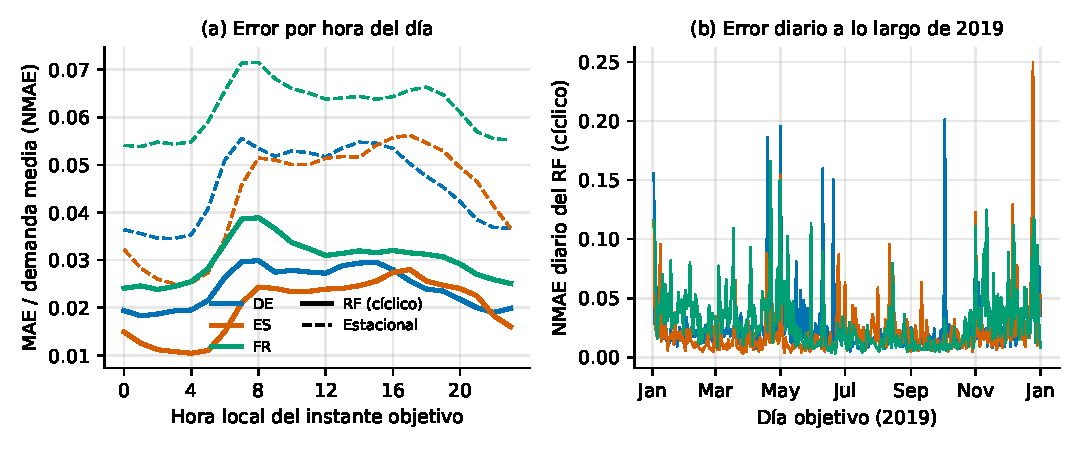
\includegraphics[width=0.86\textwidth]{img/fig_diagnostico.pdf}
\end{figure}

\begin{table}[!htbp]
    \centering
        \caption{Error del Random Forest cíclico en 2019 por subgrupo: tamaño ($n$), MAE (MW) y reducción del MAE frente a la referencia semanal.\label{tab:diag}}
        \footnotesize
        \resizebox{\textwidth}{!}{\begin{tabular}{lrrrrrrrrr}
\toprule
 & \multicolumn{3}{c}{DE} & \multicolumn{3}{c}{ES} & \multicolumn{3}{c}{FR} \\
\cmidrule(lr){2-4}\cmidrule(lr){5-7}\cmidrule(lr){8-10}
Subgrupo & $n$ & MAE RF & Mejora & $n$ & MAE RF & Mejora & $n$ & MAE RF & Mejora \\
\midrule
Laborable & 6\,240 & 1\,489 & 49\% & 6\,240 & 656 & 54\% & 6\,111 & 1\,679 & 54\% \\
Fin de semana & 2\,496 & 1\,022 & 39\% & 2\,496 & 401 & 53\% & 2\,448 & 1\,493 & 44\% \\
\midrule
Invierno & 2\,136 & 1\,549 & 54\% & 2\,136 & 763 & 52\% & 2\,136 & 2\,293 & 55\% \\
Primavera & 2\,207 & 1\,659 & 41\% & 2\,207 & 464 & 56\% & 2\,207 & 2\,034 & 38\% \\
Verano & 2\,208 & 1\,086 & 50\% & 2\,208 & 617 & 52\% & 2\,031 & 879 & 55\% \\
Otoño & 2\,185 & 1\,132 & 41\% & 2\,185 & 492 & 56\% & 2\,185 & 1\,256 & 57\% \\
\midrule
Alta ($>$ p90) & 882 & 1\,415 & 49\% & 796 & 741 & 59\% & 782 & 2\,350 & 60\% \\
Resto & 7\,854 & 1\,349 & 47\% & 7\,940 & 567 & 53\% & 7\,777 & 1\,553 & 50\% \\
\bottomrule
\end{tabular}}
    \\ Alta demanda: respuesta sobre el percentil 90 de entrenamiento de cada país.
\end{table}

El modelo supera a la referencia en las 24 horas de los tres países (figura \ref{img:diagnostico}a), con menor error de madrugada y máximos entre las 8 y las 17 h. La ventaja se mantiene en laborables y fines de semana y en las cuatro estaciones, con reducciones del MAE de 38\,\% a 57\,\%; las menores son primavera en Francia (38\,\%), fin de semana en Alemania (39\,\%) y primavera en Alemania (41\,\%). En horas de alta demanda la reducción es de 49\,\% en DE, 59\,\% en ES y 60\,\% en FR, pero el modelo \textbf{subestima} (sesgo medio de $-745$, $-456$ y $-920$ MW): quien dimensione capacidad con él quedaría corto justo cuando la demanda es mayor.

\textbf{Extremos y situación no confiable.} Los peores días son feriados nacionales (anexo, tabla \ref{tab:peores}): el MAE diario llega a 3\,700--11\,200 MW entre los tres peores de cada país, y el modelo los sobreestima (figura \ref{img:diagnostico}b). El 2 de enero en los tres países y el 26 de diciembre en Francia, también entre los peores, se subestiman, de acuerdo con que el modelo usa la demanda deprimida del día anterior. En feriados la referencia semanal tampoco es confiable y a veces es mejor (1 de mayo y 11 de noviembre en Francia; 6 de diciembre en España). \emph{Por tanto, no se recomienda confiar en la predicción para feriados ni para el día siguiente a uno prolongado.} Si faltan horas dentro de las últimas 168, no hay media móvil semanal y no puede emitirse la predicción (1,4\,\% de las filas del periodo de desarrollo, 2015--2018).
